\documentclass[a4paper,11pt]{article}

\usepackage{graphicx}
\usepackage{subfig,hyperref}
\newcommand{\HRule}{\rule{\linewidth}{0.5mm}}

\begin{document}
\pagenumbering{alph}
\begin{titlepage}
\begin{center}

\textsc{\LARGE CMSC726 Machine Learning}\\[1.5cm]

\textsc{\Large Project 2}\\[0.5cm]

\HRule \\[0.5cm]

{ \huge \bfseries Complex Classification}\\[0.4cm]

\HRule \\[1.5cm]

{\large Angjoo Kanazawa, Ran Liu, and Austin Myers}

\vfill

{\large November 1, 2011}

\end{center}
\end{titlepage}
%\title{ML CS726 Fall'11 Project 2 Complex Classifiers}
%\author{Angjoo Kanazawa, Ran Liu, Austin Myers}
%\maketitle
\pagenumbering{arabic}

\section{PCA and Kernel PCA}
\subsection{WU1}
\textsf{Depending exactly on your random data, one or more of these lines might not pass exactly through the data as we would like it to. Why not?}\\


\subsection{WU2}
\textsf{Plot the normalized eigenvalues (include the plot in your writeup). How many eigenvectors do you have to include before you've accounted for 90\% of the variance? 95\%? (Hint: see function cumsum.)}\\

% \begin{figure}[!ht]
%   \begin{center}
%   \caption{Plot of the normalized eigenvalues}
%   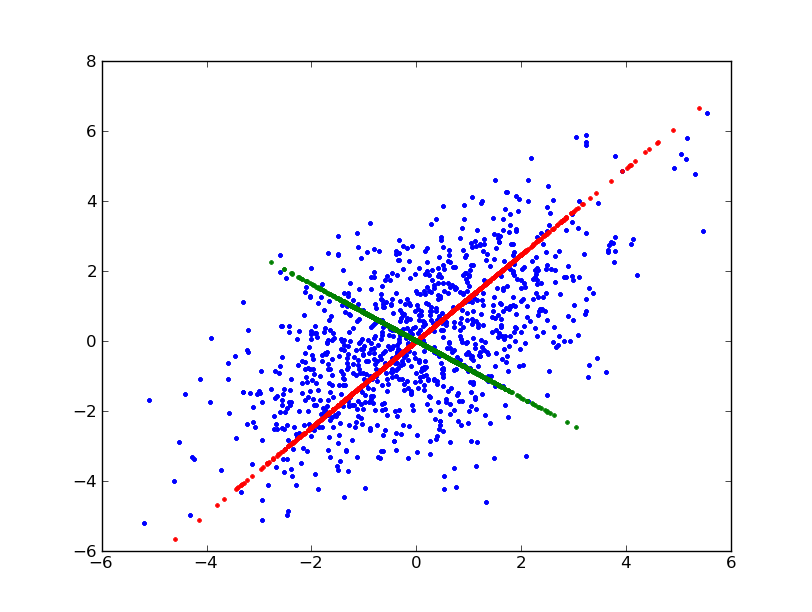
\includegraphics[width=4.5in]{pca.png}
%   \label{figures:wu61}
%   \end{center}
% \end{figure}

\subsection{WU3}
\textsf{Do these look like digits? Should they? Why or why not?
(Include the plot in your write-up.)}
% \begin{figure}[!ht]
%   \begin{center}
%   \caption{Plot of digits using vanilla pca}
%   \includegraphics[width=4.5in]{pca_digits.png}
%   \label{figures:wu61}
%   \end{center}
% \end{figure}
\subsection{WU4}
\textsf{Why does vanilla PCA find this data difficult? What is the
significance of the relatively large value of the eigenvalues here?}
\subsection{WU5}
\textsf{Did PCA do what we might want it to? Why or why not? Include
the plot to justify your answer.}
% \begin{figure}[!ht]
%   \begin{center}
%   \caption{Pca doing what we want..}
%   \includegraphics[width=4.5in]{pca2.png}
%   \label{figures:wu61}
%   \end{center}
% \end{figure}
\subsection{WU6}
\textsf{How do the eigenvalues here compare to the linear case? What
does this tell you? How does the plot look? How might this be useful
for supervised learning?}
% \begin{figure}[!ht]
%   \begin{center}
%   \caption{Using KPCA}
%   \includegraphics[width=4.5in]{pca2.png}
%   \label{figures:wu61}
%   \end{center}
% \end{figure}
\subsection{WU7}
\textsf{Experiment with different kernels, and perhaps interpolations of different kernels. Try to find a kernel that gets as much of the variance on the first two principle components as possible. Report your kernel and a plot of the data projected into 2d under that kernel.}
\pagebreak
\section{HMMs:Viterbi}
\subsection{WU8}
\textsf{find two different observation sequences of length four that
differ only in one place, but differ in more than one place in the
guessed output.}
hmm.viterbi(array([0,1,1,1]), a, b, pi) # 0 0 0 0
hmm.viterbi(array([0,1,2,1]), a, b, pi) # 0 0 1 1

\section{HMMs:Forward-backward}
\subsection{WU9}
\textsf{Why does EM settle in this configuration? What is it saying? What happens when you use three states instead of two? What's the resulting probability of the data? What about four states? What happens and why?}\\

\end{document}
